\documentclass[12pt, a4paper]{article}
\usepackage{caption}
\usepackage{float}
\usepackage{enumitem}
\usepackage{amsmath}
\usepackage{booktabs}
\usepackage{ctex}
\usepackage{url}
\usepackage{graphicx}
\usepackage{listings}
\usepackage{geometry}
\usepackage{multirow}
\usepackage{fancyhdr}
\usepackage{xcolor}
\usepackage{titlesec}
\usepackage{titletoc}
\usepackage{makecell}
\usepackage{abstract}
\usepackage{subfigure}
\usepackage{diagbox}
\usepackage{pdfpages}
\usepackage{type1cm}
\usepackage{amsfonts}
\usepackage[colorlinks,linkcolor=black,anchorcolor=black,citecolor=blue,CJKbookmarks=True]{hyperref}
\geometry{left=2cm,right=2cm,top=2cm,bottom=2cm}
\renewcommand{\contentsname}{\centering{\heiti\zihao{3}{目 \qquad 录}}}
\renewcommand{\refname}{\centerline{参考文献}}
\renewcommand\figurename{图}
\renewcommand\tablename{表}
\renewcommand\abstractname{{\large{摘要}}}
\newcommand{\tabincell}[2]{\begin{tabular}{@{}#1@{}}#2\end{tabular}}

\usepackage{pifont}  
\usepackage[perpage,symbol*]{footmisc}  
\DefineFNsymbols{circled}{{\ding{192}}{\ding{193}}{\ding{194}}  
	{\ding{195}}{\ding{196}}{\ding{197}}{\ding{198}}{\ding{199}}{\ding{200}}{\ding{201}}}  
\setfnsymbol{circled}  

\usepackage{titlesec} %自定义多级标题格式的宏包
\usepackage{zhnumber}
\titleformat{\section}{\centering\Large\bfseries}{第{\chinese{section}}章}{1em}{}

\begin{document}
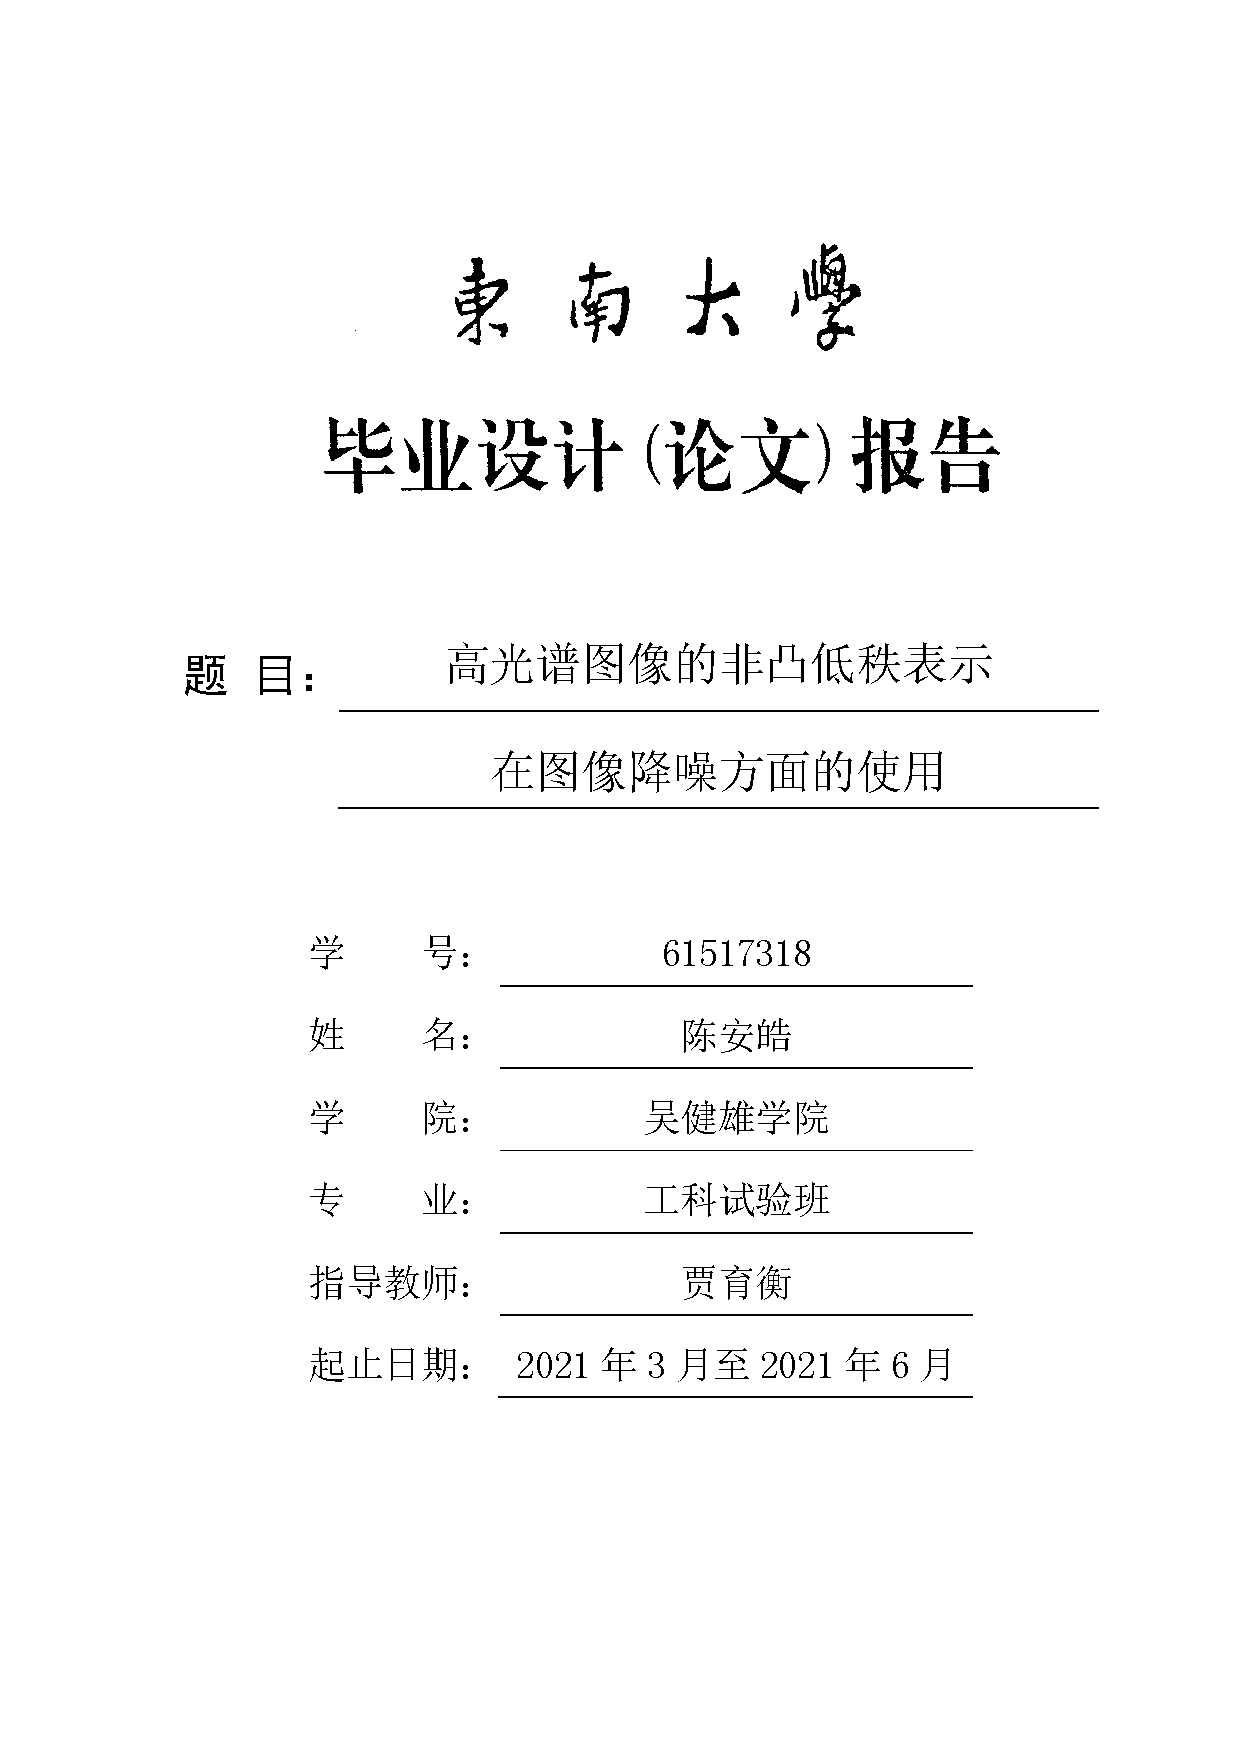
\includepdf[pages={1,2}]{cover.pdf}
	
\pagenumbering{Roman}
\begin{center}
{\Large{\bf{摘 \quad 要}}}
\end{center}
\par 高光谱遥感技术利用成像光谱仪,在几十乃至几百个窄波段同时对地物成像,因而高光谱图像含有非常丰富的空间光谱信息。这使得高光谱图像在环境、军事等诸多领域都有着十分广泛的应用。然而,由于外界的自然环境存在着复杂的电磁干扰、自身的成像设备存在着测量误差,实际采集到的高光谱图像常含有较复杂的混合噪声,包括但不限于高斯噪声、椒盐噪声以及死线噪声。这不仅会影响目视效果,而且对后续应用也会产生很大的影响。因此,对高光谱图像进行降噪是预处理阶段必不可少的步骤。
\par 对高光谱图像的降噪主要是利用了图像本身的低秩特性。由于基于秩最小化的降噪方法是一个NP-hard问题,最初,研究人员使用秩函数的凸近似,也就是核范数,去替代秩函数。尽管基于核范数最小化的降噪方法已经被应用于很多方面,它还是存在忽略奇异值的实际含义等方面的缺点。近年来,研究人员提出了一些对秩函数的非凸的放缩方式,并将其应用在图像降噪、矩阵补全等实际问题上。对这方面的研究路线可被概括成:提出对秩函数的放缩方式、建立最优化模型、求解模型。
\par 本文首先回顾了一些其他研究人员提出的、秩函数的非凸放缩方法,包括截断式核范数、权重式核范数等。在回顾了对高光谱图像降噪的研究路线之后,本文通过对人造数据与真实数据进行实验,对比了不同放缩方法的降噪效果。此外,本文还对高光谱图像降噪的未来研究方向,以及低秩特性在其他领域的应用进行了讨论。
\\
\newline
关键字:高光谱图像,非凸,低秩,核范数,降噪
\newpage
\begin{center}
{\Large{\bf{Abstract}}}
\end{center}
\par Hyper-spectral remote sensing technology takes use of imaging spectrometers to image ground objects in tens to hundreds of bands. As a result, Hyper-spectral image contains abundant spatial spectral information, making it be wildly used in environment, military, agriculture, and so on. Nevertheless, as hyper-spectral image is taken in such a natural environment where electromagnetic interference exists, hyper-spectral image humans can obtain contains several kinds of noise, including Gaussian noise, salt and pepper noise, deadlines, and so on. Not to mention that the imaging equipments are not as precise as they should be. Hyper-spectral images with noise can not only degrade the visual effect, but also do harm to their further use. Therefore, it is necessary to denoise these noised hyper-spectral images before their use.
\par When it comes to denoising hyper-spectral image, the low-rank character of natural image is mainly used by researchers. However, the denoising method which is based on Rank Minimization is a NP-hard problem. In this case, researchers tried to use nuclear norm, the convex relaxation to rank function, as the surrogate to rank function. Although this method which is based on Nuclear Norm Minimization has been wildly applied in many fields, it has some shortcomings, such as ignoring the physical meaning of different singular values. Several kinds of non-convex relaxation to rank function have been proposed in these years, and have been applied to some fields like Matrix Completion. The ideas of these paper can be concluded as: propose a new relaxation first, construct the corresponding optimization model later, and solve the model at last.
\par At the commence of this paper, several kinds of relaxation to rank function are reviewed. Later, this paper presents the experiment result on synthetic data and real visual data, in order to make comparison of denoising effect between different kinds of relaxation. In addition, this paper makes discussion of the future research direction, as well as the application of low-rank character in other fields.
\newline
\par KEY WORDS: Hyper-Spectral Image, non-convex, low rank, nuclear norm, denoising
\newpage
{{\tableofcontents}}
\newpage
\pagenumbering{arabic}
\pagestyle{fancy}
\lhead{}
\chead{东南大学本科毕业设计(论文)}
\rhead{}
\section{研究背景及意义}
\subsection{高光谱图像及其成像原理}
\par 高光谱图像(Hyper-Spectral Image, HSI),又称“高光谱分辨率遥感图像”(Hyper-Spectral Resolution Remote Sensing Image)。遥感(Remote Sensing),是在不接触目标的情况下,利用特定装置来获得地物的光谱特征信息、并对其进行提取与分析,以便能够投入到实际应用中去的一种技术\cite{whatishsi}。高光谱遥感(Hyperspectral  Remote Sensing)技术利用成像光谱仪,记录地物在太阳照射下所产生的辐射信号,在可见光以及多数红外波段等电磁波谱范围内,以非常狭窄的间隔进行成像(如图\ref{img-pricipleofphotograph}所示),进而形成不同地物的光谱特征曲线。更具体地,高光谱遥感概念的定义基础是成像光谱学,成像光谱仪作为一种遥感仪器,则可以将成像传感器的空间表示与光谱仪的分析能力结合起来,为每个像素所含有的地物提供其在上百个窄波段上的反射信息,进而得到一条完整的光谱特征曲线\cite{howtogenanhsi}。
\begin{figure}[h]
\centering
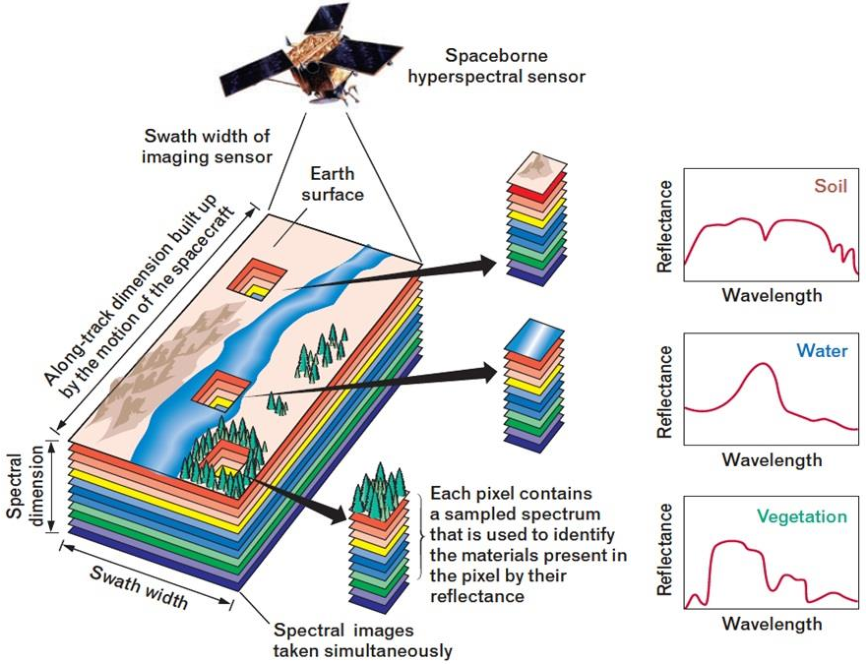
\includegraphics[scale=0.4]{img-principleofphotograph.png}
\caption{高光谱图像的成像原理}
{\scriptsize{(图片来源:{\url{https://d3i71xaburhd42.cloudfront.net/26ffa240d824f1503f3afafdc14e4a1711449138/2-Figure1-1.png}})}}
\label{img-pricipleofphotograph}
\end{figure}
\subsection{高光谱图像的特征}\label{introduction-feature}
\par 高光谱图像将地物的空间分布信息与光谱特征信息结合在一起,即:在二维空间分布信息的基础上添加了一维光谱特征信息。因此,高光谱图像可以被看成是一个立方体形式的数据:如图\ref{img-characterofphotograph}所示,每个波段都是一幅二维的平面图像,而每个像素点都是一条光谱特征曲线。由于不同物质在相同波段内的辐射强度不同,不同物质在高光谱图像中会表现出不同的光谱特征曲线\cite{howtogenanhsi},如图\ref{img-pricipleofphotograph}所示。通过对地物的连续成像,高光谱图像具有多而窄的波段,因此包含了丰富的光谱特征信息。
\begin{figure}[h]
\centering
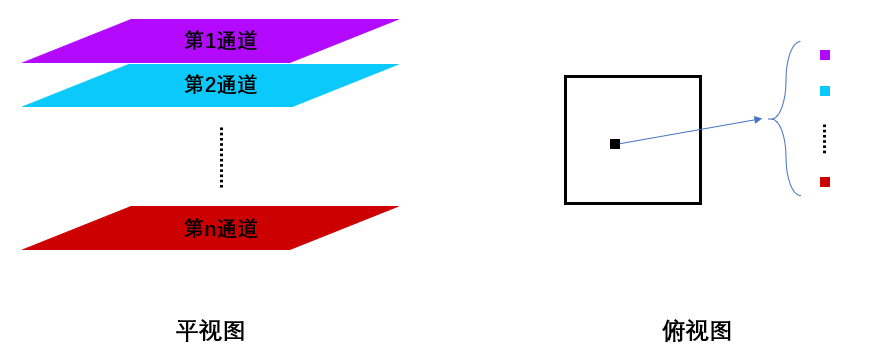
\includegraphics[scale=0.8]{img-characterofphotograph.png}
\caption{高光谱图像的特征}
\label{img-characterofphotograph}
\end{figure}
\subsection{高光谱图像的应用领域}
\par 通过纳米级的光谱分辨率,高光谱遥感技术利用成像光谱仪在几十乃至几百个窄波段同时对地物成像,因而高光谱图像含有非常丰富的空间光谱信息。这使得高光谱图像在环境、军事等诸多领域都有着十分广泛的应用\cite{usageofhsi-1}\cite{usageofhsi-2}\cite{usageofhsi-3},具体可见表\ref{usageofhsi}。
\begin{table}[H]
\centering
\caption{高光谱图像的应用领域}
\label{usageofhsi}
\begin{tabular}{ c c }
\toprule
应用领域&具体方向\\
\toprule
农业&环境监测、虫灾预报、作物估产等\\
\hline
环境&污染的监测、受灾程度的评估、自然灾害的预防等\\
\hline
地学&矿床的勘探、地形与地貌的测定、地图绘制等\\
\hline
军事&伪装物的识别、目标检测与跟踪、侦察与探测等\\
\bottomrule
\end{tabular}
\end{table}
\subsection{对高光谱图像进行降噪的意义}
\par 然而,由于外界的自然环境存在着复杂的电磁干扰、自身的成像设备存在着测量误差,实际采集到的高光谱图像常含有较复杂的混合噪声,包括但不限于高斯噪声、椒盐噪声以及死线噪声。这不仅会影响目视效果,而且对后续应用也会产生很大的影响,比如高光谱图像的分类\cite{further-use-1}、 解混\cite{further-use-2},以及目标检测\cite{further-use-3} 等。因此,对高光谱图像进行降噪是预处理阶段必不可少的步骤。
\newpage
\section{图像降噪的相关工作}\label{research-route}
\par 假设一幅一维图像$Y$受到噪声的污染,即:
\begin{equation}
\centering
Y = X + N
\label{ori-equation}
\end{equation}
式中,$X$代表未受到污染的、干净的图像,$X \in \mathbb{R}^{m \times n}$;$N$代表噪声,$N \in \mathbb{R}^{m \times n}$;$Y$代表成像设备获取到的图像,即受到污染的图像,$Y \in \mathbb{R}^{m \times n}$。
\par 那么,图像降噪的工作就是将$Y$复原为$X$。
\begin{figure}[H]
\centering
\subfigure[自然图像——贝加尔湖图]{
	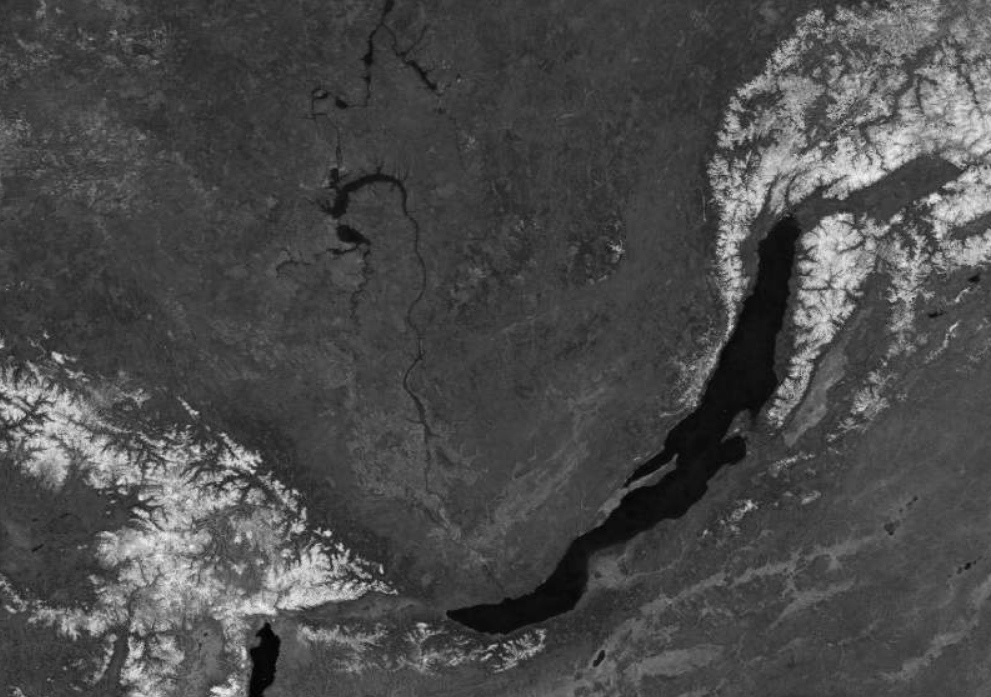
\includegraphics[scale=0.19]{x.png}
	\label{svd-example-a}
}
\subfigure[(a)图的奇异值分布图]{
	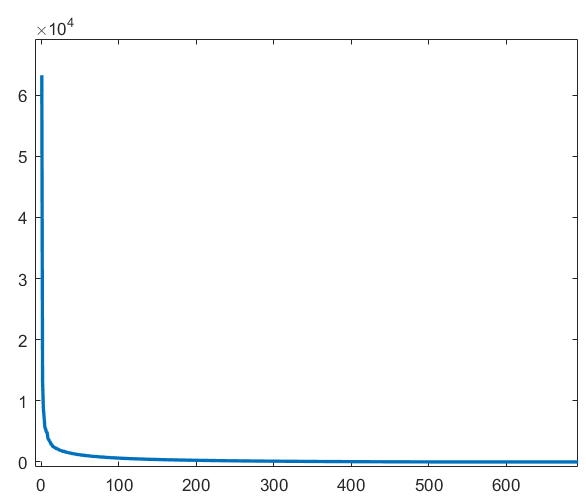
\includegraphics[scale=0.39]{y.png}
	\label{svd-example-b}
}

\caption{自然图像的低秩特性}
\label{svd-example}
\end{figure}
\par 自然图像中含有大量相似的部分。以图\ref{svd-example-a}为例,水体与水体之间、植被与植被之间、雪原与雪原之间都是相似的。因此自然图像具有低秩的特性,这一点可以被如图\ref{svd-example-b}所示的奇异值分布图证明。由于自然图像通常被认为是低秩的数据\footnote{低秩结构意味着蕴含有组合性信息。}\cite{TNN-1},基于低秩(Low Rank, LR)假设的图像降噪方法可以被形式化为:
\begin{equation}
\centering
arg\min\limits_{X} \quad rank(X)
\label{Rank-equation}
\end{equation}
式中,$rank()$代表秩函数,$rank(X)$在数值上等于矩阵$X$的秩,下同。
\par 但是,在对高光谱图像进行降噪时,既需要去除图像里的噪声,同时也需要尽可能地保留原来的信息\cite{log-norm},故拥有最小秩的矩阵并非是实际应用中所需要的\cite{log-norm}。因此,实际上,需要求解的最优化问题并非是式\ref{Rank-equation},而是:
\begin{equation}
\centering
arg\min\limits_{X} \quad \left\|Y-X\right\|_F^2 + \lambda \cdot rank(X)
\label{F-rank}
\end{equation}
式中,$X$代表未受到污染的、干净的图像,$X \in \mathbb{R}^{m \times n}$;$N$代表噪声,$N \in \mathbb{R}^{m \times n}$;$Y$代表成像设备获取到的图像,即受到污染的图像,$Y \in \mathbb{R}^{m \times n}$;$\left\|*\right\|_F$表示$Frobenius$范数;$\lambda$是正则化参数。
\par 式\ref{Rank-equation}(或式\ref{F-rank})是基于秩最小化(Rank Minimization, RM)的降噪方法,然而,这是一个NP-hard问题\cite{TNN-1}。况且,秩函数($rank()$)是不连续的\cite{TNN-1}。所以,通常使用秩函数的凸近似,也就是核范数,作为式\ref{Rank-equation} 中秩函数的替代\cite{TNN-1},即:
\begin{equation}
\centering
rank(X) \approx \left\|X\right\|_*
\label{NN-equation}
\end{equation}
式中,$\left\|*\right\|_*$代表核范数,$\left\|X\right\|_* = \sum\limits_{i=1}^{n}\sigma_i(X)$,$\sigma_i(X)$表示矩阵$X$的第$i$个奇异值。
\par 尽管式\ref{NN-equation}所示的核范数最小化(Nuclear Norm Minimization, NNM)方法已经在很多领域被成功地应用了,它还是存在缺点的。主要在于它平等地对待了所有的奇异值,即所有的奇异值都被同等程度地缩小了\cite{Review}。但是,作为先验知识,所有的奇异值都具有实际的物理含义。以降噪问题为例,有效信息通常体现在较大的奇异值中,而噪声往往隐藏在较小的奇异值中。因此,不同大小的奇异值不应该被同等地对待\cite{WNN-1}。不同于式\ref{NN-equation}的凸放缩,近些年,有研究者提出了一些非凸的放缩。
\par 考虑到如前文所述的核范数的缺点,Zhang、Hu等研究者认为,可以考虑仅仅缩小较小的奇异值\cite{TNN-1}。因此,他们提出了截断式核范数(Truncated Nuclear Norm, TNN)。截断式核范数仅仅处理较小的$n-r$个奇异值,也就是:
\begin{equation}
\centering
rank(X) \approx \left\|X\right\|_{tr,*}
\label{TNN-equation}
\end{equation}
式中,$\left\|*\right\|_{tr,*}$代表截断式核范数,$\left\|X\right\|_{tr,*} = \sum\limits_{i=r+1}^{n}\sigma_i(X)$,$\sigma_i(X)$表示矩阵$X$的第$i$个奇异值。
\par Gu等学者认为,截断式核范数因为只能做二值化选择而显得不够灵活\cite{WNN-1}。为了增加灵活性,Gu等人提出了权重式核范数(Weighted Nuclear Norm, WNN)。权重式核范数为每一个奇异值赋予了一个权重,即:
\begin{displaymath}
\centering
\left\|X\right\|_{w,*} = \sum\limits_{i=1}^{n}w_i\sigma_i(X)
\end{displaymath}
式中,$\left\|*\right\|_{w,*}$代表权重式核范数,$W=\{w_1, w_2, w_3, \cdots, w_{n-1}, w_{n}\}$是赋予不同奇异值的权重,$\sigma_i(X)$表示矩阵$X$的第$i$个奇异值。
\par 因此,秩函数被放缩为:
\begin{equation}
\centering
rank(X) \approx \left\|X\right\|_{w,*}
\label{WNN-equation}
\end{equation}
\par 在做了大量的实验后,研究人员发现这些非凸的方法比核范数表现更好。但是,Nie等学者认为,不论是截断式核范数,还是权重式核范数,又或者是阀值式核范数(Capped Nuclear Norm, CNN)\cite{CNN-1}\cite{CNN-2},都有一些不足\cite{log-norm}。 一者,它们都含有需要被事先确定的额外参数,例如截断式核范数中的$r$、 权重式核范数中的$w_i$、阀值式核范数中的$\theta$。再者,由于是非凸的放缩,求解对应的模型需要使用迭代的方法,但这些迭代的方法收敛得很慢。针对这两点不足,Nie等人提出了$log$-核范数(Log Nuclear Norm, LNN)。当秩函数被放缩为$log$-核范数后:
\begin{equation}
\centering
rank(X) \approx \left\|X\right\|_{log,*}
\label{log-equation}
\end{equation}
式中,$\left\|*\right\|_{log,*}$代表$log$-核范数,$\left\|X\right\|_{log,*} = \sum\limits_{i=1}^{n}log(\sigma_i(X)+1)$,$\sigma_i(X)$表示矩阵$X$的第$i$个奇异值。
\par 综上所述,无论是(普通)核范数,还是截断式核范数、权重式核范数,又或者是$log$-核范数,它们都是对秩函数的替代(surrogate),或称放缩(relaxation)。它们的几何意义如图\ref{surrogate-to-rank}所示。
\begin{figure}[h]
\centering
\subfigure[对秩函数的近似]{
	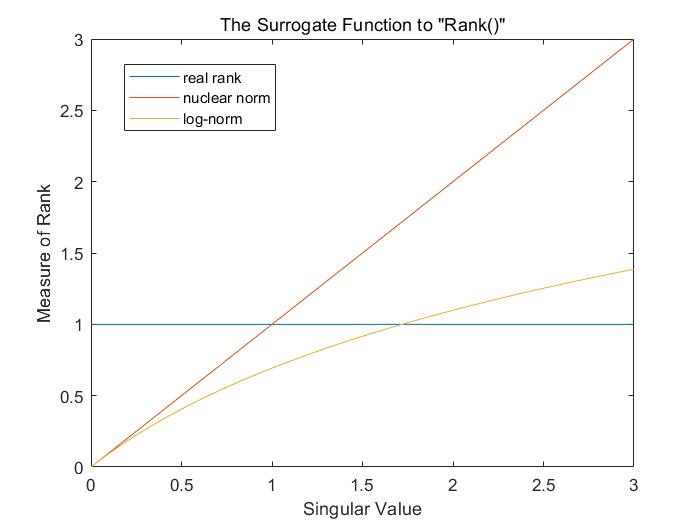
\includegraphics[scale=0.4]{surrogate-to-rank-1.png}
}
\subfigure[被处理的奇异值]{
	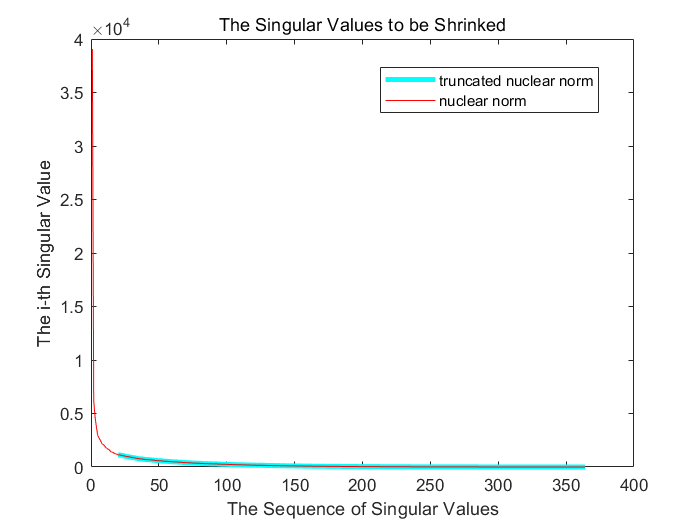
\includegraphics[scale=0.4]{surrogate-to-rank-2.png}
}

\caption{不同放缩的几何意义}
\label{surrogate-to-rank}
\end{figure}
\par 此外,还有很多种放缩方式,这里不再一一赘述,可参考表\ref{relaxation}\cite{Review}。
\begin{table}[H]
\centering
\caption{秩函数的不同放缩(部分)}
\label{relaxation}
		
\begin{tabular}{c c}
\toprule
名称&表达式\\
\toprule
核范数&$\sum\limits_{i=1}^{n}\sigma_i$\\
\hline
截断式核范数&$\sum\limits_{i=r+1}^{n}\sigma_i$\\
\hline
权重式核范数&$\sum\limits_{i=1}^{n}w_i\sigma_i$\\
\hline
阀值式核范数&$\sum\limits_{i=r+1}^{n}min(\sigma_i, \theta)$\\
\hline
$log$-核范数&$\sum\limits_{i=1}^{n}log(\sigma_i+1)$\\
\hline
$\gamma$-核范数&$\sum\limits_{i=1}^{n}\cfrac{(1+\gamma)\sigma_i}{\gamma+\sigma_i}$\\
\hline
格曼&$\sum\limits_{i=1}^{n}\cfrac{\sigma_i}{\sigma_i + \gamma}$\\
\hline
拉普拉斯&$\sum\limits_{i=1}^{n}\left(1-exp(-\cfrac{\sigma_i}{\gamma})\right)$\\
\bottomrule
\end{tabular}
\end{table}
\par 由表\ref{relaxation},可发现这些放缩都可以被抽象成如下的形式:
\begin{displaymath}
\centering
rank(X) \approx \sum\limits_{i=1}^{n}f(\sigma_i(X))
\end{displaymath}
式中,$f$代表着某种运算;$\sigma_i(X)$表示矩阵$X$的第$i$个奇异值。
\newpage
\section{研究路线}\label{related-work}
%\par 本章将具体分析第\ref{research-route}章中提到的几种核范数的替代函数在高光谱图像降噪问题中的作用。
%\par 在对高光谱图像进行降噪时,既需要去除图像里的噪声,同时也需要尽可能地保留原图信息\cite{log-norm}。因此,实际上,需要求解的最优化问题并非是式\ref{Rank-equation},而是:
%\begin{equation}
%\centering
%arg\min\limits_{X} \quad \left\|Y-X\right\|_F^2 + \lambda \cdot rank(X)
%\label{F-rank}
%\end{equation}
%式中,
%\par$X$代表未受到污染的、干净的图像;
%\par$N$代表噪声;
%\par$Y$代表成像设备获取到的图像,即受到污染的图像;
%\par$\left\|*\right\|_F$表示$Frobenius$范数;
%\par$\lambda$是正则化参数。
%\par 同理,式\ref{NN-equation}、\ref{TNN-equation}、\ref{WNN-equation}、\ref{log-equation} 也需要更新为形如式\ref{F-rank}的最优化方程。
\subsection{高光谱图像降噪的相关研究}
\par 已有的高光谱图像降噪算法主要归纳为两类。
\par 一类是基于空间维的降噪算法。此类算法从人类的视觉角度出发,将高光谱图像的每个波段视为灰度图像,直接应用数字图像处理领域中的、已经发展得较为成熟的图像降噪算法对高光谱图像进行逐波段降噪。这类算法的典型代表有:非局部均值算法(Non-Local Mean, NLM)\cite{NLM}、总变分模型(Total Variation, TV)\cite{TV}、高斯混合模型(Gaussian Mixture Model, GMM)\cite{GMM}、基于小波变换的三维块匹配快速降噪算法(Block-Matching and 3D filtering, BM3D)\cite{BM3D},以及本文第\ref{research-route} 章提到的几种核范数最小化模型。此类算法应用方式简单,但是,大多算法也仅限于对传统二维图像降噪算法的简单应用和推广,侧重于从空间维对高光谱图像的单个波段进行去噪。然而,空间维的信息不能充分地反映高光谱图像的全部信息,基于空间维的降噪算法忽略了高光谱图像波段间的高度相关性。对高光谱图像所有波段进行逐降噪不仅计算复杂度高,而且由于没有考虑到光谱维的相关性。本章所述的几种降噪方法可以被归类到这一类方法中去。
\par 另一类是基于联合空间-光谱维的降噪算法。为了充分利用空间维和光谱维的高度相关性,除空间维外,这一类算法考虑到了光谱维的相关性。例如,光谱-空间自适应总变分模型(Spectral–Spatial Adaptive Hyperspectral Total Variation, SSAHTV)\cite{SSAHTV}提出:在空间维中,算法对每一个像素的降噪强度应根据不同地物类型进行自适应调节,同样在光谱维中,算法对每一个波段的降噪强度也应根据不同波段的噪声强度进行自适应调节。\cite{BM4D}和\cite{VBM4D}是基于BM3D算法提出的对图像序列或者视频降噪的BM4D和VBM4D算法,在高光谱图像降噪中,这两个算法将高光谱图像立方体视为图像序列或视频进行降噪。MSPCA-BM3D\cite{MSPCA-BM3D}提出通过非局部(non-local)空间自适应和光谱维去相关对多光谱或高光谱图像进行降噪。PCA+BM4D\cite{PCAplusBM4D}首先对有噪声的高光谱数据进行主成分变换,保持前几个信号能量高的主成分不变,使用BM4D算法对剩余信号低能量的主成分进行降噪\cite{yaodan}。
\subsection{本章安排}
\par 在第\ref{research-route}章,本文给出了多种基于低秩假设的一维图像降噪方法。对高光谱图像的降噪可以采用“分治”的策略:高光谱图像的每一个通道都可以视为一张一维图像,对这些一维图像分别进行降噪处理,最后再将那些去噪后的一维图像按原本的顺序拼成一张高维图像,那么这张高维图像即是降噪后的高光谱图像。本章的剩余部分将具体分析第\ref{research-route}章中提到的几种核范数的替代函数在高光谱图像降噪问题中的作用,也就是如何使用这些核范数的替代函数对一幅二维图像进行降噪。
\subsection{使用核范数替代秩函数的降噪方法}
\par 由于式\ref{F-rank}是一个NP-hard问题,加之秩函数是不连续的。因此,通常使用秩函数的凸近似,即核范数,替代式\ref{F-rank}中秩函数的部分。所以,式\ref{F-rank}更新为:
\begin{equation}
\centering
arg\min\limits_{X} \quad \left\|Y-X\right\|_F^2 + \lambda \cdot \left\|X\right\|_*
\label{F-nn}
\end{equation}
式中,$X$代表未受到污染的、干净的图像,$X \in \mathbb{R}^{m \times n}$;$N$代表噪声,$N \in \mathbb{R}^{m \times n}$;$Y$代表成像设备获取到的图像,即受到污染的图像,$Y \in \mathbb{R}^{m \times n}$;$\left\|*\right\|_F$表示$Frobenius$范数;$\lambda$是正则化参数;$\left\|*\right\|_*$代表(标准)核范数,$\left\|X\right\|_* = \sum\limits_{i=1}^{n}\sigma_i(X)$,$\sigma_i(X)$表示矩阵$X$的第$i$个奇异值。
\subsection{使用截断式核范数替代秩函数的降噪方法}
\par 若使用截断式核范数替代式\ref{F-rank}中秩函数的部分,则式\ref{F-rank}被更新为:
\begin{equation}
\centering
arg\min\limits_{X} \quad \left\|Y-X\right\|_F^2 + \lambda \cdot \left\|X\right\|_{tr,*}
\label{F-tnn}
\end{equation}
式中,$X$代表未受到污染的、干净的图像,$X \in \mathbb{R}^{m \times n}$;$N$代表噪声,$N \in \mathbb{R}^{m \times n}$;$Y$代表成像设备获取到的图像,即受到污染的图像,$Y \in \mathbb{R}^{m \times n}$;$\left\|*\right\|_F$表示$Frobenius$范数;$\lambda$是正则化参数;$\left\|*\right\|_{tr,*}$代表截断式核范数,$\left\|X\right\|_{tr,*} = \sum\limits_{i=r+1}^{n}\sigma_i(X)$,$r$是其中的参数,$\sigma_i(X)$表示矩阵$X$的第$i$个奇异值。
\subsection{使用权重式核范数替代秩函数的降噪方法}
\par 由于截断式核范数对所有奇异值做的是两极化选择,因此会显得不够灵活。而权重式核范数则是针对这一点所做的改进。如果使用权重式核范数替代式\ref{F-rank}中秩函数的部分,则式\ref{F-rank} 被更新为:
\begin{equation}
\centering
arg\min\limits_{X} \quad \left\|Y-X\right\|_F^2 + \lambda \cdot \left\|X\right\|_{w,*}
\label{F-wnn}
\end{equation}
式中,$X$代表未受到污染的、干净的图像,$X \in \mathbb{R}^{m \times n}$;$N$代表噪声,$N \in \mathbb{R}^{m \times n}$;$Y$代表成像设备获取到的图像,即受到污染的图像,$Y \in \mathbb{R}^{m \times n}$;$\left\|*\right\|_F$表示$Frobenius$范数;$\lambda$是正则化参数;$\left\|*\right\|_{w,*}$代表权重式核范数,$\left\|X\right\|_{w,*} = \sum\limits_{i=1}^{n}w_i\sigma_i(X)$,$\sigma_i(X)$表示矩阵$X$的第$i$个奇异值,$W=\{w_1, w_2, w_3, \cdots, w_{n-1}, w_{n}\}$是赋予不同奇异值的权重\footnote{并且可以证明,$W$是非降的。}。
\subsection{使用$log$-核范数替代秩函数的降噪方法}
\par 考虑到无论是截断式核范数,还是权重式核范数,都包含额外的参数,而这些额外的参数需要在事先被确定。这就给很多实际应用带来了麻烦。$log$-核范数则不包含额外的参数。基于$log$-核范数,式\ref{F-rank}被更新为:
\begin{equation}
\centering
arg\min\limits_{X} \quad \left\|Y-X\right\|_F^2 + \lambda \cdot \left\|X\right\|_{log,*}
\label{F-lnn}
\end{equation}
式中,$X$代表未受到污染的、干净的图像,$X \in \mathbb{R}^{m \times n}$;$N$代表噪声,$N \in \mathbb{R}^{m \times n}$;$Y$代表成像设备获取到的图像,即受到污染的图像,$Y \in \mathbb{R}^{m \times n}$;$\left\|*\right\|_F$表示$Frobenius$范数;$\lambda$是正则化参数;$\left\|*\right\|_{log,*}$代表$log$-核范数,$\left\|X\right\|_{log,*} = \sum\limits_{i=1}^{n}log(\sigma_i(X)+1)$,$\sigma_i(X)$表示矩阵$X$的第$i$个奇异值。

\subsection{本章小结}
\par 本章主要分析了第\ref{research-route}章中提到的几种核范数的替代函数在高光谱图像降噪问题中的作用,也就是如何使用这些核范数的替代函数对一幅二维图像进行降噪。
\par 综合式\ref{F-nn}、\ref{F-tnn}、\ref{F-wnn}、\ref{F-lnn},实际应用中求解的最优化方程可抽象成:
\begin{displaymath}
\centering
arg\min\limits_{X} \quad \left\|Y-X\right\|_F^2 + \lambda \cdot \sum\limits_{i=1}^{n}f(\sigma_i(X))
\end{displaymath}
式中,$X$代表未受到污染的、干净的图像,$X \in \mathbb{R}^{m \times n}$;$N$代表噪声,$N \in \mathbb{R}^{m \times n}$;$Y$代表成像设备获取到的图像,即受到污染的图像,$Y \in \mathbb{R}^{m \times n}$;$\left\|*\right\|_F$表示$Frobenius$范数;$\lambda$是正则化参数;$f$代表着某种运算;$\sigma_i(X)$表示矩阵$X$的第$i$个奇异值。
\newpage
\section{实验部分}\label{experiment}
\begin{itemize}
\item 本文的全部代码:{\url{https://github.com/AnhaoROMA/matrix-denoising-by-lowrank.git}}
\item 实验环境:MATLAB R2021b
\item 实验配置:
\par 设备名称:Lenovo LAPTOP-06D3M7TP
\par 处理器:Intel(R) Core(TM) i7-7700HQ CPU @2.80GHz 2.81GHz
\par 操作系统:Microsoft Windows 10 家庭中文版
\end{itemize}
\subsection{评价降噪效果的指标——峰值信噪比}
\par 给定一个大小为$m \times n$的干净图像$I$和它的含噪图像$K$,它们的均方误差(Mean Square Error, MSE)为:
\begin{displaymath}
\centering
MSE = \cfrac{1}{mn}\sum_{i=1}^{m}\sum_{j=1}^{n}\left(I_{i,j}-K_{i, j}\right)^2
\end{displaymath}
\par 那么它们的峰值信噪比(Peak Signal-to-Noise Ratio, PSNR)就是:
\begin{displaymath}
\centering
PSNR = 10 \times log_{10}\left(\cfrac{MAX^2}{MSE}\right)
\end{displaymath}
式中,
\par$MAX$指图像可能的最大像素值,对由$B$位二进制表示的图像来说,$MAX=2^B-1$。
\par 不难发现,图像$M$和图像$N$之间的PSNR值愈大,$M$与$N$在直观上愈相近。因此,从含噪图像$K$恢复出的降噪图像$I'$,$I'$与干净图像$I$ 之间的PSNR值越大,说明降噪的效果越好。
	% \par 事实上,除了峰值信噪比,结构相似性(Structural SIMilarity, SSIM)也可以量化降噪效果。因本文篇幅有限,故在此不作讨论。
\subsection{实验设计}
\par 与一般的RGB图像只含有R、G、B三个通道不同,高光谱图像的通道数量众多。以Urban数据集\footnote{数据来源:\url{http://www.tec.army.mil/hypercube}}为例,Urban数据集内的图像规格为:$304 \times 304 \times 210$,即图像包含210个通道。因此,想目视高光谱图像,通常只取其中某一通道,而不选择同时直接目视全部通道。基于这点限制,本文的实验分为两个部分。
\subsubsection{人造数据部分}\label{synthetic}
\par 一是对普通的一维图像进行降噪。这部分可根据需要,任意地给无噪声图像添加特定种类的噪声,被人为添加特定噪声后的实验用图像在其他研究人员的论文中被称作人造数据(Synthetic Data)。本文将通过计算降噪后的图像与无噪声的原图像之间的PSNR值来量化不同降噪方法的效果。
\subsubsection{真实视觉数据部分}\label{real}
\par 二是对真实的、自然获取到的高光谱图像进行降噪。这部分的实验用图像均是在生产实践中获取的,在其他研究人员的论文中被称为真实视觉数据(Real Visual Data),由于无法获取它们的无噪声的原图像,加之无法同时显示所有通道,故仅能展示其中某些通道经过不同降噪方法后得到的去噪图像,用于目视效果的对比。由于高光谱图像通常不是8bit图,故在展示某一通道的图像之前,还需要进行像素值的映射,将高位图转为一般的8 位图。
\subsection{实验数据}
\par \ref{synthetic}节的实验数据如下:
\begin{itemize}
\item 实验0
\par 图\ref{syn-data-0}:不含噪声的原图像
		
\item 实验1
\par 图\ref{syn-data-1}:含方差为0.1的零均值高斯噪声的图像
		
\item 实验2
\par 图\ref{syn-data-2}:含方差为0.5的零均值高斯噪声的图像
		
\item 实验3
\par 图\ref{syn-data-3}:含方差为1的零均值高斯噪声的图像
		
\item 实验4
\par 图\ref{syn-data-4}:含方差为5的零均值高斯噪声的图像

\item 实验5
\par 图\ref{syn-data-5}:含5\%椒盐噪声的图像
\item 实验6
\par 图\ref{syn-data-6}:含10\%椒盐噪声的图像
\item 实验7
\par 图\ref{syn-data-7}:含20\%椒盐噪声的图像
\item 实验8
\par 图\ref{syn-data-8}:含40\%椒盐噪声的图像

\item 实验9
\par 图\ref{syn-data-9}:含10\%椒盐噪声与方差为0.1的零均值高斯噪声的图像
\item 实验10
\par 图\ref{syn-data-10}:含10\%椒盐噪声与方差为1的零均值高斯噪声的图像
\item 实验11
\par 图\ref{syn-data-11}:含20\%椒盐噪声与方差为1的零均值高斯噪声的图像
\end{itemize}

\begin{figure}[h]
\centering
\subfigure[无噪声的原图]{
	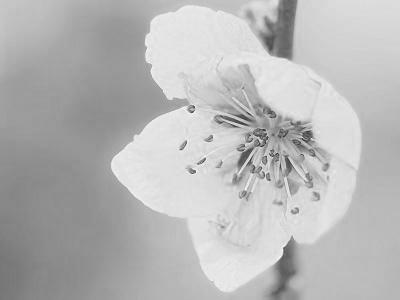
\includegraphics[scale=0.25]{exp-0.jpg}
	\label{syn-data-0}
}
\subfigure[含方差为0.1的零均值高斯噪声的图像]{
	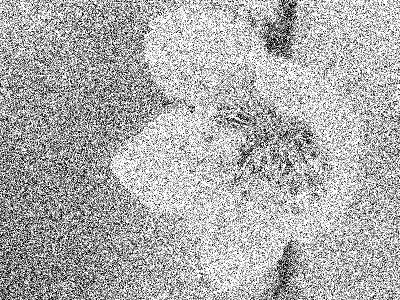
\includegraphics[scale=0.25]{exp-1.jpg}
	\label{syn-data-1}
}
\subfigure[含方差为0.5的零均值高斯噪声的图像]{
	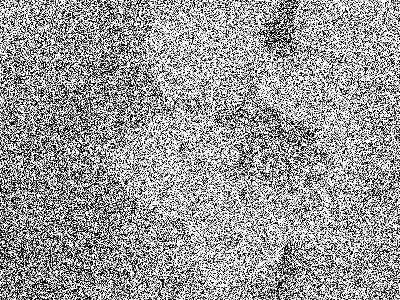
\includegraphics[scale=0.25]{exp-2.jpg}
	\label{syn-data-2}
}
\subfigure[含方差为1的零均值高斯噪声的图像]{
	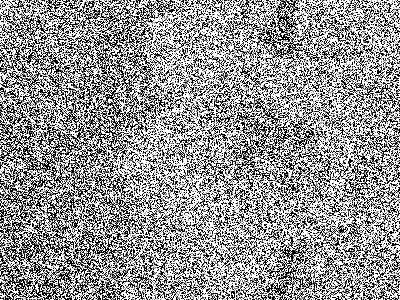
\includegraphics[scale=0.25]{exp-3.jpg}
	\label{syn-data-3}
}
		
\subfigure[含方差为5的零均值高斯噪声的图像]{
	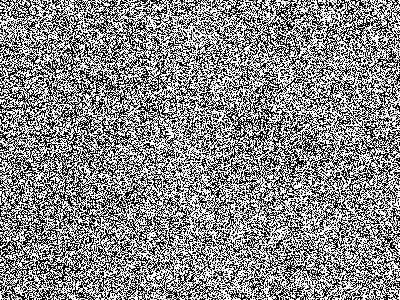
\includegraphics[scale=0.25]{exp-4.jpg}
	\label{syn-data-4}
}
\subfigure[含5\%椒盐噪声的图像]{
	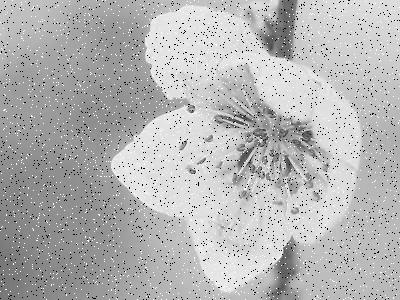
\includegraphics[scale=0.25]{exp-5.jpg}
	\label{syn-data-5}
}
\subfigure[含10\%椒盐噪声的图像]{
	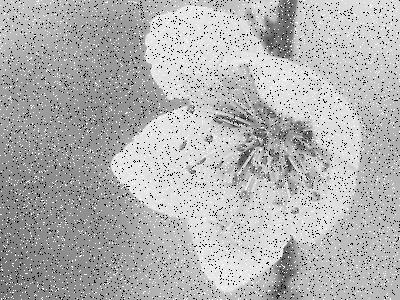
\includegraphics[scale=0.25]{exp-6.jpg}
	\label{syn-data-6}
}
\subfigure[含20\%椒盐噪声的图像]{
	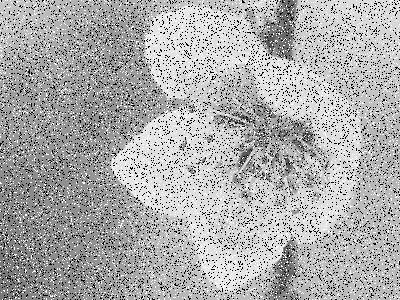
\includegraphics[scale=0.25]{exp-7.jpg}
	\label{syn-data-7}
}
\subfigure[含40\%椒盐噪声的图像]{
	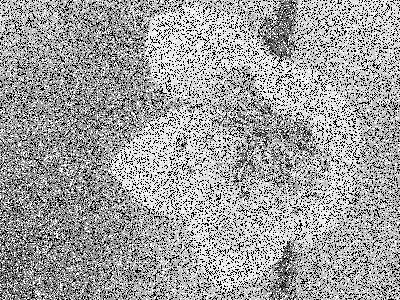
\includegraphics[scale=0.25]{exp-8.jpg}
	\label{syn-data-8}
}
\subfigure[含10\%椒盐噪声与方差为0.1的零均值高斯噪声的图像]{
	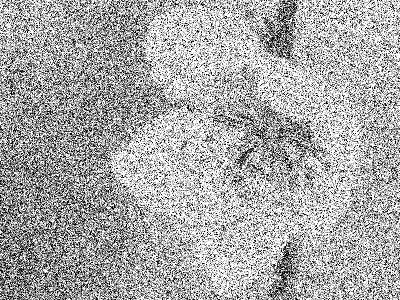
\includegraphics[scale=0.25]{exp-9.jpg}
	\label{syn-data-9}
}
\subfigure[含10\%椒盐噪声与方差为1的零均值高斯噪声的图像]{
	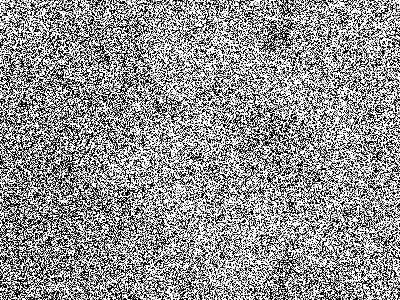
\includegraphics[scale=0.25]{exp-10.jpg}
	\label{syn-data-10}
}
\subfigure[含20\%椒盐噪声与方差为1的零均值高斯噪声的图像]{
	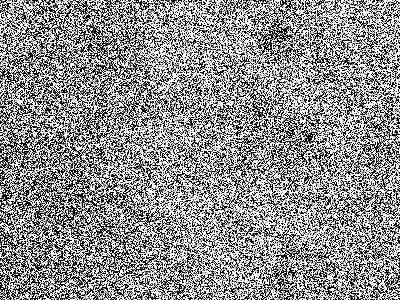
\includegraphics[scale=0.25]{exp-11.jpg}
	\label{syn-data-11}
}

\caption{人造数据}
\label{syn-data}
\end{figure}
	
\par \ref{real}节的实验数据如下:
\begin{itemize}
\item 实验12
\par 图\ref{real-data}:Urban数据集内的一幅图像
\end{itemize}

\begin{figure}[h]
\centering
\subfigure[高光谱图像的第2通道]{
	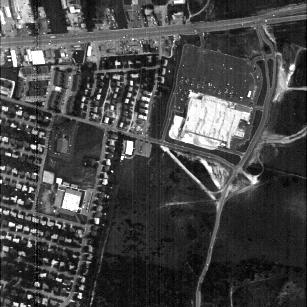
\includegraphics[scale=0.6]{band-2.jpg}
	\label{band-2}
}
\subfigure[高光谱图像的第103通道]{
	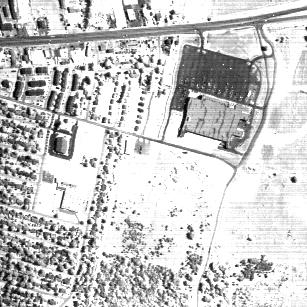
\includegraphics[scale=0.6]{band-103.jpg}
	\label{band-103}
}
		
\subfigure[高光谱图像的第187通道]{
	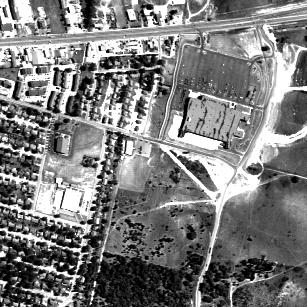
\includegraphics[scale=0.6]{band-187.jpg}
	\label{band-187}
}
\subfigure[高光谱图像的第189通道]{
	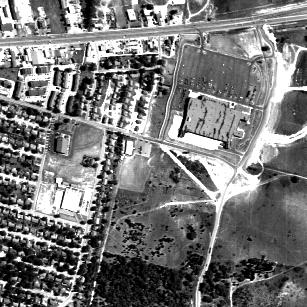
\includegraphics[scale=0.6]{band-189.jpg}
	\label{band-189}
}
		
\caption{真实视觉数据}
\label{real-data}
\end{figure}

\subsection{实验结果与分析}\label{analysis}
\subsubsection{人造数据部分的实验结果}
\par 为了体现降噪的直观效果,本文以基于权重式核范数的降噪方法为例,图\ref{syn-data-1}$\sim$图\ref{syn-data-11}经降噪处理后的结果分别见图\ref{Screenshot_1}$\sim$图\ref{Screenshot_11}。
\begin{figure}[htbp]
\centering
		
\subfigure[含方差为0.1的零均值高斯噪声的图像经降噪处理后的结果]{
	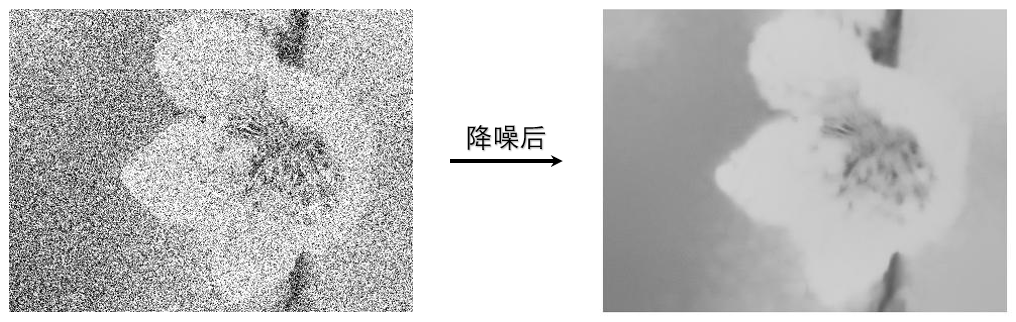
\includegraphics[scale=0.35]{Screenshot_1.png}
	\label{Screenshot_1}
}
\subfigure[含方差为0.5的零均值高斯噪声的图像经降噪处理后的结果]{
	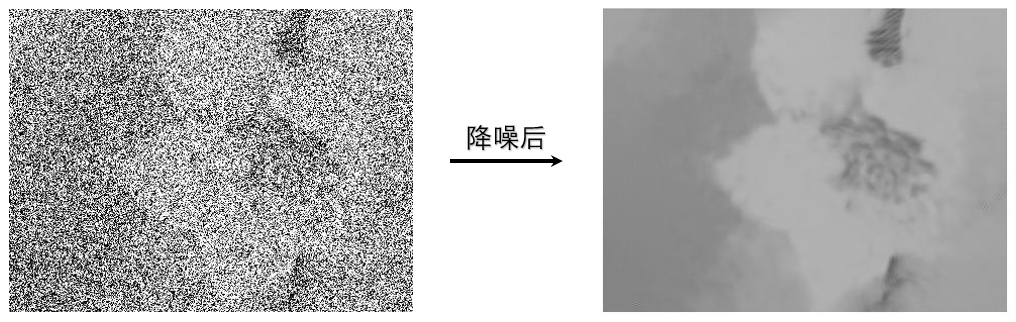
\includegraphics[scale=0.35]{Screenshot_2.png}
	\label{Screenshot_2}
}
		
\subfigure[含方差为1的零均值高斯噪声的图像经降噪处理后的结果]{
	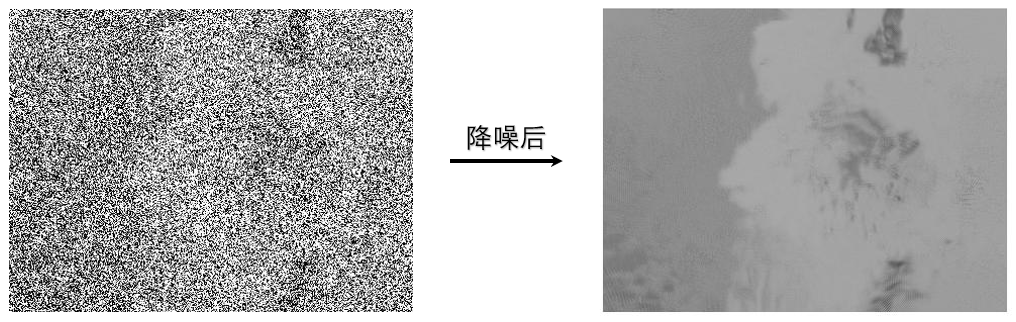
\includegraphics[scale=0.35]{Screenshot_3.png}
	\label{Screenshot_3}
}
\subfigure[含方差为5的零均值高斯噪声的图像经降噪处理后的结果]{
	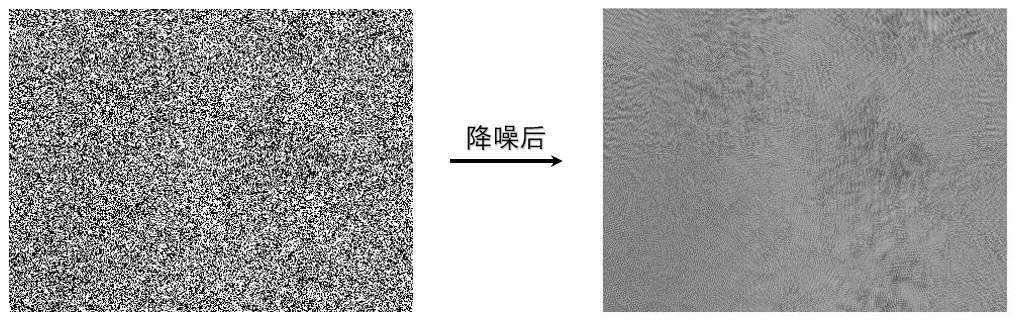
\includegraphics[scale=0.35]{Screenshot_4.png}
	\label{Screenshot_4}
}
		
\subfigure[含5\%椒盐噪声的图像经降噪处理后的结果]{
	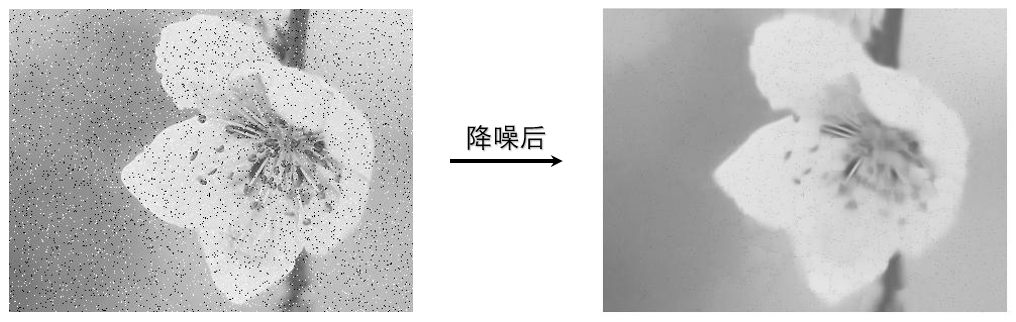
\includegraphics[scale=0.35]{Screenshot_5.png}
	\label{Screenshot_5}
}
\subfigure[含10\%椒盐噪声的图像经降噪处理后的结果]{
	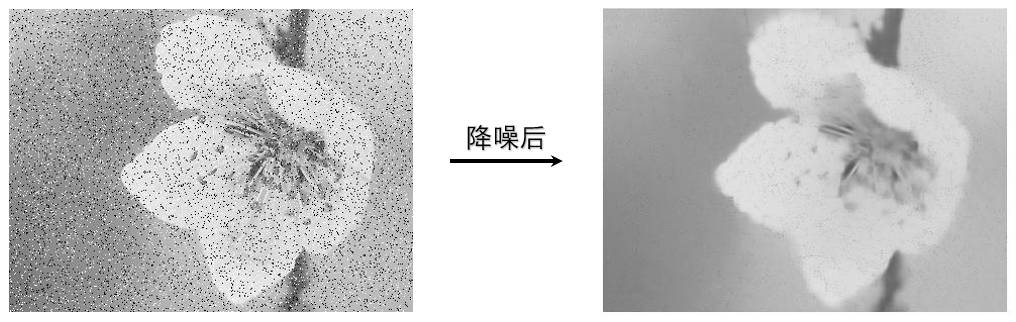
\includegraphics[scale=0.35]{Screenshot_6.png}
	\label{Screenshot_6}
}
		
\subfigure[含20\%椒盐噪声的图像经降噪处理后的结果]{
	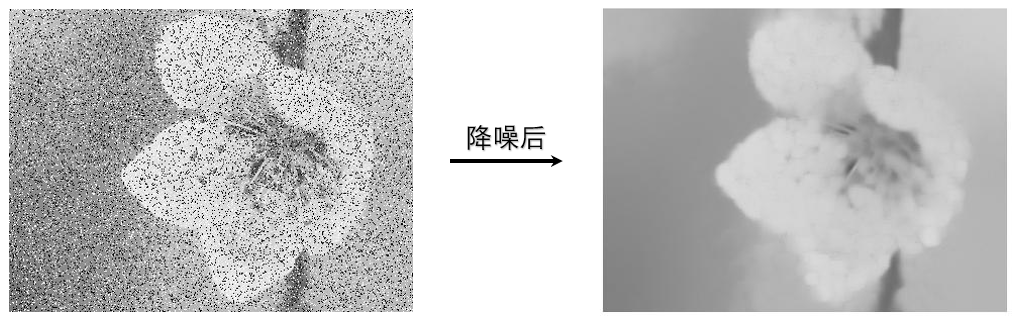
\includegraphics[scale=0.35]{Screenshot_7.png}
	\label{Screenshot_7}
}
\subfigure[含40\%椒盐噪声的图像经降噪处理后的结果]{
	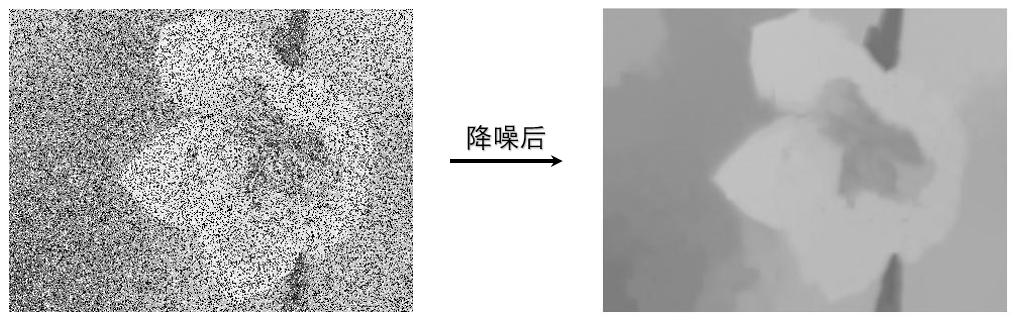
\includegraphics[scale=0.35]{Screenshot_8.png}
	\label{Screenshot_8}
}
		
\subfigure[含10\%椒盐噪声与方差为0.1的零均值高斯噪声的图像]{
	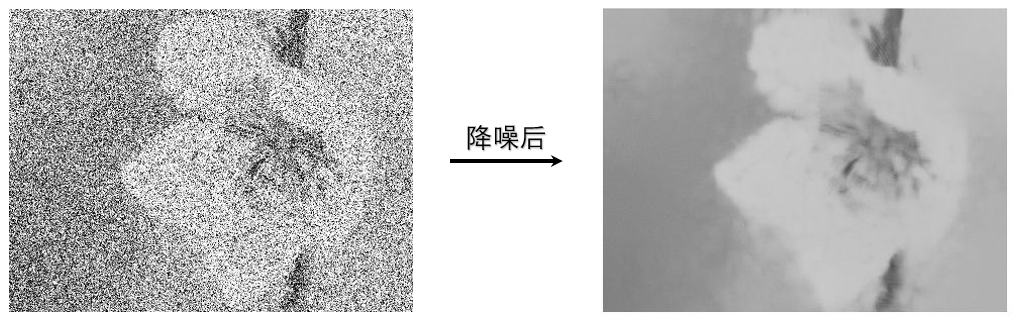
\includegraphics[scale=0.35]{Screenshot_9.png}
	\label{Screenshot_9}
}
\subfigure[含10\%椒盐噪声与方差为1的零均值高斯噪声的图像]{
	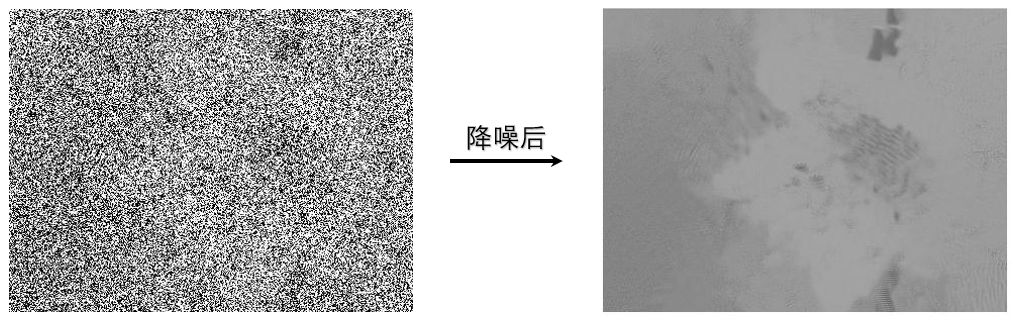
\includegraphics[scale=0.35]{Screenshot_10.png}
	\label{Screenshot_10}
}
		
\subfigure[含20\%椒盐噪声与方差为1的零均值高斯噪声的图像]{
	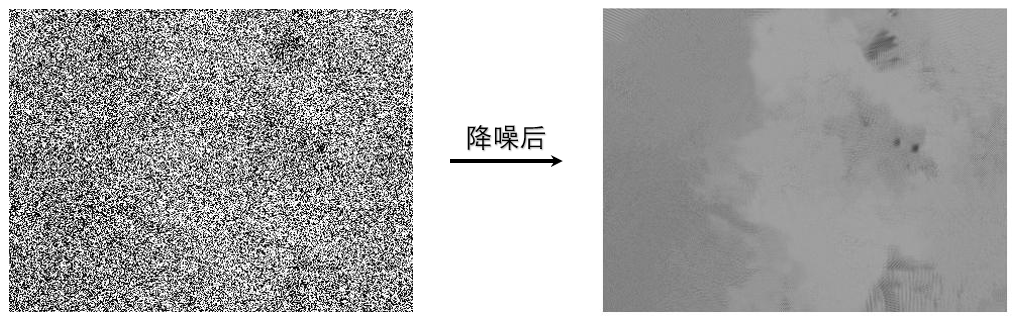
\includegraphics[scale=0.35]{Screenshot_11.png}
	\label{Screenshot_11}
}
		
\caption{经基于权重式核范数的降噪方法处理后的结果}
\label{Screenshot}
\end{figure}
\par 此外,为了对比不同的降噪方法的降噪效果,本文用第\ref{related-work}章中提到的四种方法对所有的人造数据进行了测试,实验结果见表\ref{exp-res}。
	
\begin{table}[h]
\centering
\caption{用不同的降噪方法对不同的图像进行降噪处理的效果}
\label{exp-res}
\begin{tabular}{|c|c|c|c|c|}
\hline
\diagbox{待降噪图像}{PSNR值}{降噪方法} & 核范数 & 权重式核范数 & $log$-核范数 & 截断式核范数 \\
\hline
% \makecell[居中情况]{第1行内容 \\ 第2行内容 \\ 第3行内容 ...} & 1 & 2 & 3 & 4 \\
\makecell[c]{含方差为0.1的零均\\ 值高斯噪声的图像} & 20.81 & {\bf{25.01}} & 24.86 & 20.91 \\
\hline
\makecell[c]{含方差为0.5的零均\\ 值高斯噪声的图像} & 16.61 & {\bf{18.08}} & 18.00 & 16.67 \\
\hline
\makecell[c]{含方差为1的零均\\ 值高斯噪声的图像} & 14.80 & {\bf{16.24}} & 16.11 & 14.87 \\
\hline
\makecell[c]{含方差为5的零均\\ 值高斯噪声的图像} & 12.98 & 13.28 & {\bf{13.56}} & 12.97 \\
\hline
含5\%椒盐噪声的图像 & 24.80 & {\bf{29.76}} & 29.17 & 24.84 \\
\hline
含10\%椒盐噪声的图像 & 22.98 & 28.35 & {\bf{28.44}} & 23.02 \\
\hline
含20\%椒盐噪声的图像 & 20.95 & 25.90 & {\bf{25.99}} & 21.00 \\
\hline
含40\%椒盐噪声的图像 & 18.44 & {\bf{20.64}} & 20.59 & 18.48 \\
\hline
			
\makecell[c]{含10\%椒盐噪声与\\ 方差为0.1的零均值\\ 高斯噪声的图像} & 18.36 & {\bf{22.94}} & 22.83 & 18.36 \\
\hline
\makecell[c]{含10\%椒盐噪声与\\ 方差为1的零均值\\ 高斯噪声的图像} & 14.31 & {\bf{15.67}} & 15.51 & 14.38 \\
\hline
\makecell[c]{含20\%椒盐噪声与\\ 方差为1的零均值\\ 高斯噪声的图像} & 14.10 & {\bf{15.16}} & 14.99 & 14.12 \\
\hline
\end{tabular}
\end{table}
	
\subsubsection{真实视觉数据部分的实验结果}
\par 高光谱图像第2、103、187、189个通道,经不同降噪方法进行降噪处理后的结果见图\ref{bands-2}$\sim$图\ref{bands-189}。
% 2nd
\begin{figure}[htbp]
\centering		
\subfigure[经基于核范数的降噪方法]{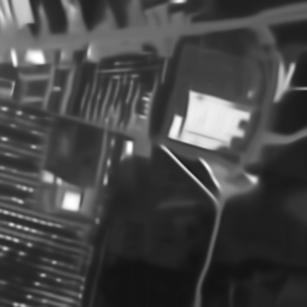
\includegraphics[scale=0.3]{band-2-NN.jpg}}
\subfigure[经基于截断式核范数的降噪方法]{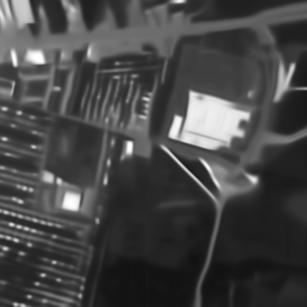
\includegraphics[scale=0.3]{band-2-TNN.jpg}}
\subfigure[经基于$log$-核范数的降噪方法]{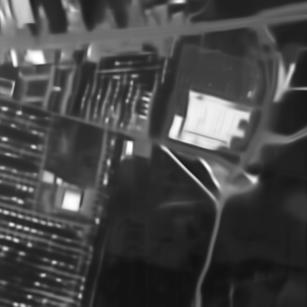
\includegraphics[scale=0.3]{band-2-LNN.jpg}}
\subfigure[经基于权重式核范数的降噪方法]{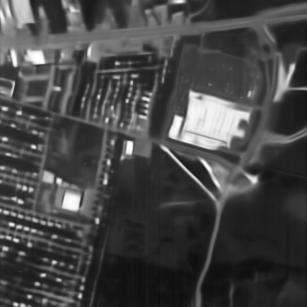
\includegraphics[scale=0.3]{band-2-WNN.jpg}}
\caption{高光谱图像的第2个通道(图\ref{band-2})经不同降噪方法进行处理的结果}
\label{bands-2}
\end{figure}
	
% 103rd
\begin{figure}[htbp]
\centering	
\subfigure[经基于核范数的降噪方法]{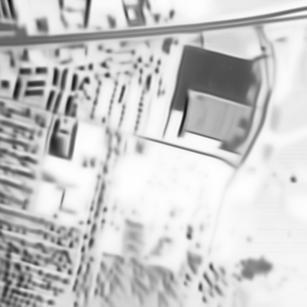
\includegraphics[scale=0.3]{band-103-NN.jpg}}
\subfigure[经基于截断式核范数的降噪方法]{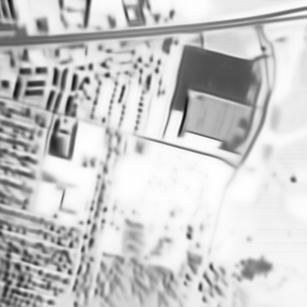
\includegraphics[scale=0.3]{band-103-TNN.jpg}}
\subfigure[经基于$log$-核范数的降噪方法]{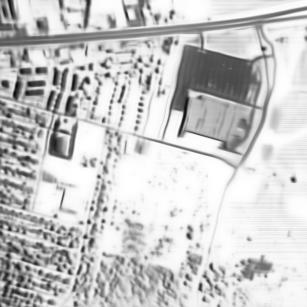
\includegraphics[scale=0.3]{band-103-LNN.jpg}}
\subfigure[经基于权重式核范数的降噪方法]{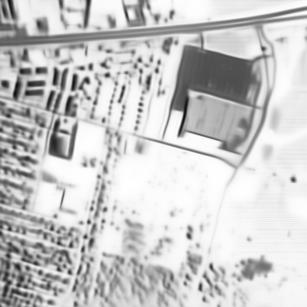
\includegraphics[scale=0.3]{band-103-WNN.jpg}}
\caption{高光谱图像的第103个通道(图\ref{band-103})经不同降噪方法进行处理的结果}
\label{bands-103}
\end{figure}
	
% 187rd
\begin{figure}[htbp]
\centering	
\subfigure[经基于核范数的降噪方法]{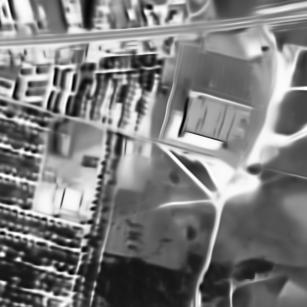
\includegraphics[scale=0.3]{band-187-NN.jpg}}
\subfigure[经基于截断式核范数的降噪方法]{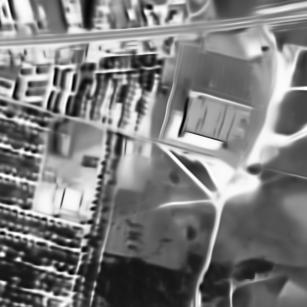
\includegraphics[scale=0.3]{band-187-TNN.jpg}}
\subfigure[经基于$log$-核范数的降噪方法]{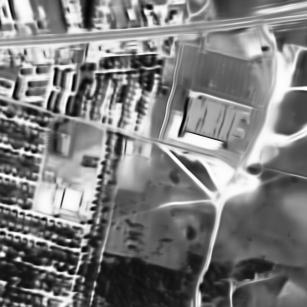
\includegraphics[scale=0.3]{band-187-LNN.jpg}}
\subfigure[经基于权重式核范数的降噪方法]{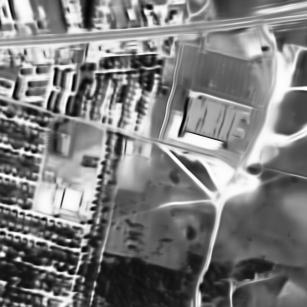
\includegraphics[scale=0.3]{band-187-WNN.jpg}}
\caption{高光谱图像的第187个通道(图\ref{band-187})经不同降噪方法进行处理的结果}
\label{bands-187}
\end{figure}
	
% 189th
\begin{figure}[htbp]
\centering
		
\subfigure[经基于核范数的降噪方法]{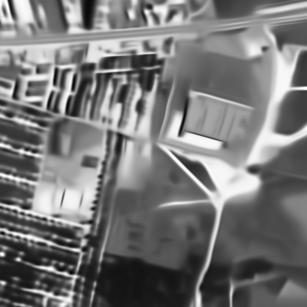
\includegraphics[scale=0.3]{band-189-NN.jpg}}
\subfigure[经基于截断式核范数的降噪方法]{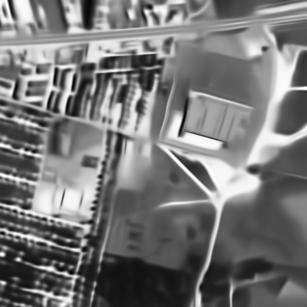
\includegraphics[scale=0.3]{band-189-TNN.jpg}}
\subfigure[经基于$log$-核范数的降噪方法]{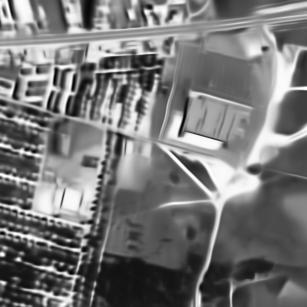
\includegraphics[scale=0.3]{band-189-LNN.jpg}}
\subfigure[经基于权重式核范数的降噪方法]{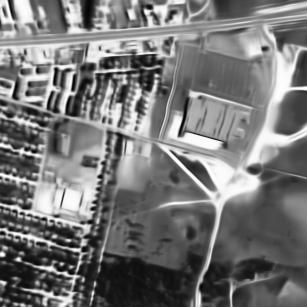
\includegraphics[scale=0.3]{band-189-WNN.jpg}}
\caption{高光谱图像的第189个通道(图\ref{band-189})经不同降噪方法进行处理的结果}
\label{bands-189}
\end{figure}
\subsubsection{结果分析}
\par 由表\ref{exp-res}及图\ref{exp-types},不难发现,基于权重式核范数与基于$log$-核范数的降噪方法比另外两种方法更加有效,这与本文第\ref{research-route}章的表述一致,即权重式核范数是针对截断式核范数的缺点所进行的改进。$log$-核范数比起权重式范数的优点在于,使用者无需事先决定权值$W=\{w_1, w_2, w_3, \cdots, w_{n-1}, w_n\}$这个额外的参数。
\begin{figure}[H]
\centering
\subfigure[不同方差的零均值高斯噪声]{\includegraphics[scale=0.3]{exp-type-gaussian.png}}
\subfigure[不同程度的椒盐噪声]{\includegraphics[scale=0.3]{exp-type-pepperandsalt.png}}
\subfigure[不同类型的混合噪声]{\includegraphics[scale=0.3]{exp-type-mixed.png}}
\caption{表\ref{exp-res}的图示}
\label{exp-types}
\end{figure}
	
\par 图\ref{bands-2}$\sim$图\ref{bands-189}是本文在自然获取的高光谱图像上做的实验。由于需要将16位图像映射成8位图像,导致显示出的8位图像的每一位都对应着$2^8=256$个可能的、真实的数值。这也是导致不同的降噪结果在目视下非常相似的原因。

\newpage
\section{未来工作展望}
\subsection{秩函数的不同放缩方法之间的相互融合}
\par 本文所述的、对秩函数的不同近似方法是相对独立的,因而可以相互结合。例如,Nie等学者将阀值式核范数(Capped Nuclear Norm)与Schatten $p$-范数结合起来,提出了Capped $Sp$-范数\cite{CNN-2}。再比如,Xie、Gu等研究人员将Schatten $p$-范数与权重式核范数结合成Weighted Schatten $p$-范数\cite{merge-2}。
\subsection{混合噪声的降噪问题}
\par 实际的高光谱图像往往被多种噪声污染,包括但不限于高斯噪声(Gaussian noise)、冲击噪声(impulse noise)、死线噪声(dead lines)、死点噪声(dead pixels)和条纹噪声(stripes)\cite{Mixture}。在第\ref{related-work}章,本文将所有的噪声统一成了$N$,这也是绝大多数文章所做的。但也有例外。例如,Zhang、He等学者用$l_1$-范数评估稀疏噪声的稀疏性,以此将稀疏噪声与高斯噪声独立开来,并由此构造了$GoDec$模型\cite{Mixture},Meng学者也对含混合噪声的低秩结构降噪问题有所涉猎\cite{meng}。但就总体来说,对混合噪声的降噪研究并不算多。
\subsection{使用张量的降噪方法}
% 空间分布信息与光谱特征信息
\par 本文所述的几种降噪方法,均是使用矩阵(Matrix)的,也就是在二维平面上降噪。这样做可以考虑到图像的空间分布特征。但是,正如第\ref{introduction-feature}节所述,高光谱图像可以看作是多层二维图像的叠加,每一层二维图像都是相同的场景在特定波段内的辐射。因此,除了每层层内的空间分布信息,各层层间还存在光谱特征信息。针对矩阵在考量光谱特征信息这方面的不足,近年来,Lu 等研究者提出了使用张量(Tensor)的降噪方法\cite{Tensor-1}\cite{Tensor-2}\cite{Tensor-3}。这方面的研究路线与矩阵的类似,都是先考虑核范数的凸放缩\cite{Tensor-1},再研究非凸放缩\cite{Tensor-2}\cite{Tensor-3}。
\subsection{低秩特性的其他应用}
\par 本文将图像视作一个低秩的数据结构,并讨论了对其的降噪问题。对低秩特性的利用还可以被用于\cite{Review}:
\begin{itemize}
\item 鲁棒的主成分分析法(Robust Principal Component Analysis)
\par 鲁棒的主成分分析法是从含噪声的观测数据中恢复一个低秩矩阵的最有效的办法之一。从数学角度出发,鲁棒的主成分分析法将含噪声的观测数据$M$视作是低秩矩阵$X$与代表噪声的矩阵$E$之和,并通过求解下式以分离出$X$与$E$。
\begin{displaymath}
\min\limits_{X,E}\quad \left\|E\right\|_1 + \lambda \cdot rank(X) \qquad s.t.\quad M=X+E
\end{displaymath}
式中,
\par$X$是低秩矩阵,$X \in \mathbb{R}^{m \times n}$;
\par$E$是代表噪声的矩阵,$E \in \mathbb{R}^{m \times n}$;
\par$M$是含噪声的观测数据,$M \in \mathbb{R}^{m \times n}$;
\par$\left\|*\right\|_1$表示$l_1$-范数,这部分可以根据需要被其他的矩阵范数替换;
\par$rank(*)$表示秩函数,这部分可以根据需要被秩函数的某一种放缩方式替代。
\item 矩阵补全(Matrix Completion)
\par 若一个矩阵$M$含有缺失的元素,那么矩阵补全的任务就是利用矩阵$M$中的已知元素去推测缺失的元素,以此达到补全矩阵的效果。常用的矩阵补全方法也是利用了原矩阵的低秩性,即事先假设了原矩阵是低秩或近似低秩的。矩阵补全的问题可以被形式化成:
\begin{displaymath}
\min\limits_{X}\quad \left\|X-M\right\|_1 + \lambda \cdot rank(X) \qquad s.t.\quad M_{i,j}=X_{i,j}, (i,j)\in\Omega
\end{displaymath}
式中,
\par$X$代表不含缺失元素的原矩阵,$X \in \mathbb{R}^{m \times n}$;
\par$M$代表含有缺失元素的待补全的矩阵,$M \in \mathbb{R}^{m \times n}$;
\par$\Omega=\{(i,j)|1\leq i \leq m, 1\leq j \leq n\}$代表已知元素所在的位置;
\par$\left\|*\right\|_1$表示$l_1$-范数,这部分可以根据需要被其他的矩阵范数替换;
\par$rank(*)$表示秩函数,这部分可以根据需要被秩函数的某一种放缩方式替代。
% \item 多任务学习(Multi-Task Learning)
		
% \item 子空间聚类(Subspace Clustering)
		
\item 视频背景提取(Video background subtraction)
\par 视频背景提取是前文所述的鲁棒的主成分分析法的应用之一。若给定一段视频,则可以将这段视频的每一帧拼接起来,构成一个矩阵。那么,可以将视频的背景(如风景、环境等)视为主成分,将前景(如移动物体等)视为噪声。
\item 推荐系统(Recommender System)
\par 推荐系统是前文所述的矩阵补全的应用之一。如图\ref{recommender-system}所示,某些用户对某些电影打出评分,构成了评分表,但是评分表是不完整的。在使用矩阵补全方法将评分表中的缺失元素补全之后,若某用户对某电影的评分被系统预测是高分且该用户未曾观看过该电影,则系统可将该电影推送给该用户。
\begin{figure}[H]
\centering
\includegraphics[scale=0.7]{recommender-system.png}
\caption{用户对电影的评分表}
\label{recommender-system}
\end{figure}
\end{itemize}
\newpage
\section{总结}
\par 高光谱遥感技术利用成像光谱仪,在几十乃至几百个窄波段同时对地物成像,因而高光谱图像含有非常丰富的空间光谱信息。这使得高光谱图像在环境、军事等诸多领域都有着十分广泛的应用。然而,由于外界的自然环境存在着复杂的电磁干扰、自身的成像设备存在着测量误差,实际采集到的高光谱图像常含有较复杂的混合噪声,包括但不限于高斯噪声、椒盐噪声以及死线噪声。这不仅会影响目视效果,而且对后续应用也会产生很大的影响。因此,对高光谱图像进行降噪是预处理阶段必不可少的步骤。
\par 对高光谱图像的降噪主要是利用了图像本身的低秩特性。由于基于秩最小化的降噪方法是一个NP-hard问题,最初,研究人员使用秩函数的凸近似,也就是核范数,去替代秩函数。尽管基于核范数最小化的降噪方法已经被应用于很多方面,它还是存在忽略奇异值的实际含义等方面的缺点的。近几年,一些对秩函数的非凸的放缩方式被提出,并被应用于图像降噪、矩阵补全等实际问题。这些非凸放缩方式包括截断式核范数、权重式核范数、$log$-核范数、$\gamma$-核范数等。此类文章的研究思路可被概括为:提出对秩函数的放缩方式、建立最优化模型、求解模型。
\par 本文首先回顾了一些其他研究人员提出的、秩函数的非凸放缩方法,分别是截断式核范数、权重式核范数与$log$-核范数。之后,本文通过对人造数据与真实数据进行实验,对比了不同放缩方法的降噪效果,发现基于权重式核范数与$log$-核范数的降噪方法的降噪效果要优于其它两种。最后,本文对高光谱图像降噪的未来研究方向,以及低秩特性在其他领域的应用进行了讨论。
	
\newpage
\begin{thebibliography}{99}
\addcontentsline{toc}{section}{参考文献}
%\bibitem{...}...
\bibitem{whatishsi}童庆禧, 张兵, 郑兰芬.高光谱遥感——原理、技术与应用[M].高等教育出版社:北京,2006:2-10.
\bibitem{howtogenanhsi}张显.基于子空间低秩表示的高光谱图像去噪方法研究[D].南京:南京邮电大学,2020.
\bibitem{usageofhsi-1}浦瑞良, 宫鹏.高光谱遥感及其应用[M].高等教育出版社:北京,2000:48-122.
		
\bibitem{usageofhsi-2}Sarah A. Lewis, Andrew T. Hudak, Roger D. Ottmar.Using hyperspectral imagery to estimate forest floor consumption from wildfire in boreal forests of Alaska, USA[J].International Journal of Wildland Fire,2011,20(2):255-271.
		
\bibitem{usageofhsi-3}K.C. Tiwari, M.K. Arora, D. Singh.An assessment of independent component analysis for detection of military targets from hyperspectral images[J].International Journal of Applied Earth Observation and Geoinformation,2011,13(5):730-740.
		
\bibitem{further-use-1}C. Bo, H. Lu and D. Wang, "Weighted Generalized Nearest Neighbor for Hyperspectral Image Classification," in IEEE Access, vol. 5, pp. 1496-1509, 2017.
		
\bibitem{further-use-2}W. Yang, K. Hou, B. Liu, F. Yu and L. Lin, "Two-Stage Clustering Technique Based on the Neighboring Union Histogram for Hyperspectral Remote Sensing Images," in IEEE Access, vol. 5, pp. 5640-5647, 2017.
		
\bibitem{further-use-3}Lili Zhang, Chunhui Zhao.A spectral-spatial method based on low-rank and sparse matrix decomposition for hyperspectral anomaly detection[J].International Journal of Remote Sensing,2017,38(14):4047-4068.
		
\bibitem{TNN-1}D. Zhang, Y. Hu, J. Ye, X. Li and X. He, "Matrix completion by Truncated Nuclear Norm Regularization," 2012 IEEE Conference on Computer Vision and Pattern Recognition, 2012, pp. 2192-2199.
		
\bibitem{log-norm}F. Nie, Z. Hu and X. Li, "Matrix Completion Based on Non-Convex Low-Rank Approximation," in IEEE Transactions on Image Processing, vol. 28, no. 5, pp. 2378-2388, May 2019.
		
\bibitem{Review}Zhanxuan Hu, Feiping Nie, Rong Wang,etc.Low Rank Regularization: A review[J].Neural Networks,2021,136:218-232.
		
\bibitem{WNN-1}S. Gu, L. Zhang, W. Zuo and X. Feng, "Weighted Nuclear Norm Minimization with Application to Image Denoising," 2014 IEEE Conference on Computer Vision and Pattern Recognition, 2014, pp. 2862-2869. %, doi: 10.1109/CVPR.2014.366.
		
\bibitem{CNN-1}Sun Qian, Xiang Shuo, Ye Jieping. (2013). Robust principal component analysis via capped norms. 311-319. %10.1145/2487575.2487604.
		
\bibitem{CNN-2}Nie, F. et al. “Joint Capped Norms Minimization for Robust Matrix Recovery.” IJCAI (2017).
% \bibitem{merge-1}Joint capped norms minimization for robust matrix recovery.
		
\bibitem{NLM}A. Buades, B. Coll and J. -. Morel, "A non-local algorithm for image denoising," 2005 IEEE Computer Society Conference on Computer Vision and Pattern Recognition (CVPR'05), 2005, pp. 60-65 vol. 2. %, doi: 10.1109/CVPR.2005.38.
		
\bibitem{TV}Leonid I. Rudin, Stanley Osher, Emad Fatemi.Nonlinear total variation based noise removal algorithms[J].Physica D: Nonlinear Phenomena,1992,60(1):259-268.
		
\bibitem{GMM}Afonso Teodoro, Mariana Almeida, Mario Figueiredo.Single-frame Image Denoising and Inpainting Using Gaussian Mixtures[J].Proceedings of the International Conference on Pattern Recognition Applications and Methods,2015,2:283-288.
		
\bibitem{BM3D}K. Dabov, A. Foi, V. Katkovnik and K. Egiazarian, "Image Denoising by Sparse 3-D Transform-Domain Collaborative Filtering," in IEEE Transactions on Image Processing, vol. 16, no. 8, pp. 2080-2095, Aug. 2007. %, doi: 10.1109/TIP.2007.901238.
		
\bibitem{SSAHTV}Q. Yuan, L. Zhang and H. Shen, "Hyperspectral Image Denoising Employing a Spectral–Spatial Adaptive Total Variation Model," in IEEE Transactions on Geoscience and Remote Sensing, vol. 50, no. 10, pp. 3660-3677, Oct. 2012. %, doi: 10.1109/TGRS.2012.2185054.
\bibitem{BM4D}M. Maggioni, V. Katkovnik, K. Egiazarian and A. Foi, "Nonlocal Transform-Domain Filter for Volumetric Data Denoising and Reconstruction," in IEEE Transactions on Image Processing, vol. 22, no. 1, pp. 119-133, Jan. 2013. %, doi: 10.1109/TIP.2012.2210725.
\bibitem{VBM4D}M. Maggioni, G. Boracchi, A. Foi and K. Egiazarian, "Video Denoising, Deblocking, and Enhancement Through Separable 4-D Nonlocal Spatiotemporal Transforms," in IEEE Transactions on Image Processing, vol. 21, no. 9, pp. 3952-3966, Sept. 2012. %, doi: 10.1109/TIP.2012.2199324.
\bibitem{MSPCA-BM3D}Danielyan A, Foi A, Katkovnik V, et al. Denoising of multispectral images via nonlocal groupwise spectrum-PCA[C]//Conference on Colour in Graphics, Imaging, and Vision. Society for Imaging Science and Technology, 2010, 2010(1): 261-266.
\bibitem{PCAplusBM4D}CHEN G, BUI T D, QUACH K G, et al. Denoising Hyperspectral Imagery Using Principal Component Analysis and Block-Matching 4D Filtering[J]. Canadian Journal of Remote Sensing, 2014, 40(1):60–66.
		
\bibitem{yaodan}姚丹. 基于低秩表示的高光谱图像降噪和修复算法研究[D].中国科学院大学(中国科学院遥感与数字地球研究所),2018.
		
\bibitem{merge-2}Y. Xie, S. Gu, Y. Liu, W. Zuo, W. Zhang and L. Zhang, "Weighted Schatten  $p$ -Norm Minimization for Image Denoising and Background Subtraction," in IEEE Transactions on Image Processing, vol. 25, no. 10, pp. 4842-4857, Oct. 2016.%, doi: 10.1109/TIP.2016.2599290.
		
\bibitem{Mixture}H. Zhang, W. He, L. Zhang, H. Shen and Q. Yuan, "Hyperspectral Image Restoration Using Low-Rank Matrix Recovery," in IEEE Transactions on Geoscience and Remote Sensing, vol. 52, no. 8, pp. 4729-4743, Aug. 2014.%, doi: 10.1109/TGRS.2013.2284280.
		
\bibitem{meng}Xiangyong Cao, Yang Chen, Qian Zhao, Deyu Meng, Yao Wang, Dong Wang, Zongben Xu. Low-rank Matrix Factorization under General Mixture Noise DIstributions. ICCV (oral), 2015.
		
\bibitem{Tensor-1}Lu, Canyi, Jiashi Feng, Y. Chen, W. Liu, Zhouchen Lin and S. Yan. “Tensor Robust Principal Component Analysis: Exact Recovery of Corrupted Low-Rank Tensors via Convex Optimization.” 2016 IEEE Conference on Computer Vision and Pattern Recognition (CVPR) (2016): 5249-5257.
		
\bibitem{Tensor-2}S. Xue, W. Qiu, F. Liu and X. Jin, "Low-Rank Tensor Completion by Truncated Nuclear Norm Regularization," 2018 24th International Conference on Pattern Recognition (ICPR), 2018, pp. 2600-2605.%, doi: 10.1109/ICPR.2018.8546008.
		
\bibitem{Tensor-3}Liu, Hongyi, Hanyang Li, Zebin Wu and Z. Wei. “Hyperspectral Image Recovery Using Non-Convex Low-Rank Tensor Approximation.” Remote. Sens. 12 (2020): 2264.
		
\bibitem{gamma}[1]王洪雁,王拓,潘勉,汪祖民.基于伽马范数最小化的图像去噪算法[J].通信学报,2020,41(10):222-230.
\bibitem{others-1}李欢.基于低秩稀疏理论的图像去噪算法研究[D]. 南京:南京邮电大学,2018.
\end{thebibliography}
	
\newpage
%\begin{center}
%{\Large{\bf{致 \quad 谢}}}
%\end{center}
\section*{致 \quad 谢}
\addcontentsline{toc}{section}{致 \quad 谢}
\par 本论文是在贾育衡老师的悉心指导下完成的。在毕设初期,我对“高光谱图像的非凸低秩表示”这方面不甚了解,面对这方面浩如烟海的研究文献不知所措。贾老师在获悉这一情况后,帮助我概括出这类文章的写作思路。就好像醍醐灌顶一样,我逐渐理清了这方面的研究路线。接下来,我按照贾老师的建议,对收集到的论文进行了分类与总结。当我对如何撰写一篇逻辑严谨、行文流畅的论文感到困惑的时候,贾老师提纲挈领地指出文章的结构:综述、实验与分析,而这也是本论文的最终结构。除了对我在学业上的帮助,贾老师对我的不断鼓励给我提供了做好毕设的动力。在人生下一阶段的方向选择的问题上,贾老师也给出了一些建议与帮助。“夫蚊虻终日经营,不能越阶序,然附骥尾则涉千里,攀鸿鹄则翔四海。”可以想象,如果没有贾老师的帮助、仅仅依靠我自己的努力,我很难顺利地完成毕业设计。
\par 在东南大学的四年时光,将是我人生篇章里充实的一页。在这四年里,在老师、同学和朋友的陪伴下,我有着很多难忘的经历。在大一、大二,作为班长,我协助学院管理班级;在大二的寒假,我与袁华和宋晨辉两位同学组队参加2019美国大学生数学建模竞赛;在伍家松老师的指导下,我与袁华和张逸帆两位同学合作完成了一个省创SRTP项目;在SAP实习期间,我与Nanjing Branch的同事们、SAP Labs 的Francesco Di Cerbo一起工作$\cdots\cdots$ 正是这些经历,让我比起四年前更加成熟。如果没有作为班长管理班级的经历,我不会如此深刻地感受到为集体奉献的意义、作为领导者的责任与担当。虽然我在高中就背诵过《荀子$\cdot$天论》中的“君子敬其在己者,不慕其在天者”,但我从来没有真正理解过这句话,那时候我偏执地认为付出就是为了“有形的收获”。但大学四年里大大小小、或成功或失利的竞赛经历,却让我逐渐认可了在付出之后,那“无形收获”的“无用之用”,我也慢慢地学会了去坦然接受尽完全力之后的任何结果。在SRTP 项目开展期间,我与队友们通力合作,并借机提高自己的团队合作能力。在SAP实习期间,除了专业水平,我的表达能力也有了进一步的提高,而与Francesco的Sync Meeting则为我提供了宝贵的提高英文交流水平的机会。除此之外,实习期间的收入也帮助我树立了正确的金钱观与消费观。
\par 最后,我真诚地感谢母校为我提供了一个良好的成长环境、学院对我的关怀、老师们对我的指导与鼓励、同学们和朋友们对我的支持。
\end{document}
